\documentclass[a4paper,
fontsize=11pt,
%headings=small,
oneside,
numbers=noperiodatend,
parskip=half-,
bibliography=totoc,
final
]{scrartcl}

\usepackage{synttree}
\usepackage{graphicx}
\setkeys{Gin}{width=.6\textwidth} %default pics size

\graphicspath{{./plots/}}
\usepackage[ngerman]{babel}
%\usepackage{amsmath}
\usepackage[utf8x]{inputenc}
\usepackage [hyphens]{url}

\usepackage[colorlinks, linkcolor=black,citecolor=black, urlcolor=blue,
breaklinks= true]{hyperref}
\usepackage{booktabs} 
\usepackage[left=2.4cm,right=2.4cm,top=2.3cm,bottom=2cm,includeheadfoot]{geometry}
\usepackage{eurosym}
\usepackage{multirow}
\usepackage[ngerman]{varioref}
\setcapindent{1em}
\renewcommand{\labelitemi}{--}
\usepackage{paralist}
\usepackage{pdfpages}
\usepackage{lscape}
\usepackage{float}
\usepackage{acronym}
\usepackage{eurosym}
\usepackage[babel]{csquotes}
\usepackage{longtable,lscape}
\usepackage{mathpazo}
\usepackage[flushmargin,ragged]{footmisc} % left align footnote

\urlstyle{same}  % don't use monospace font for urls

\usepackage[fleqn]{amsmath}

%adjust fontsize for part

\usepackage{sectsty}
\partfont{\large}

%Das BibTeX-Zeichen mit \BibTeX setzen:
\def\symbol#1{\char #1\relax}
\def\bsl{{\tt\symbol{'134}}}
\def\BibTeX{{\rm B\kern-.05em{\sc i\kern-.025em b}\kern-.08em
    T\kern-.1667em\lower.7ex\hbox{E}\kern-.125emX}}

\usepackage{fancyhdr}
\fancyhf{}

\pagestyle{fancyplain}

\fancyhead[R]{\thepage}
%meta

\fancyhead[L]{S. Wiederkehr \\ %author
LIBREAS. Library Ideas, 24 (2014). % journal, issue, volume.
\href{http://nbn-resolving.de/urn:nbn:de:kobv:11-100215917}{urn:nbn:de:kobv:11-100215917}} % urn
\fancyhead[R]{\thepage} %page number
\fancyfoot[L] {\textit{Creative Commons BY 3.0}} %licence
\fancyfoot[R] {\textit{ISSN: 1860-7950}}

\title{\LARGE{Ein leichter Einstieg in die Geschichtswissenschaft} \\ \large{Rezension zu: Doina Oehlmann (2012): Erfolgreich recherchieren –
Geschichte (= Erfolgreich recherchieren). Berlin ; Boston MA : De
Gruyter Saur. IX, 131 S., ISBN 978-3-11-027112-6 (brosch.),
978-3-11-027130-0 (E-Book), \EUR{19,95}.}} %title %title
\author{Stefan Wiederkehr} %author

\date{}

\begin{document}

\maketitle
\thispagestyle{fancyplain} 





Der zu besprechende Band ist Teil einer neuen Reihe, mit der der Verlag
De Gruyter sich \enquote{Studierende in allen Phasen des Studiums sowie
{[}\ldots{}{]} alle wissenschaftlich interessierten Leserinnen und
Leser} als neues Zielpublikum erschließen möchte. Das Ziel, nicht nur
institutionelle Käufer, Fachreferenten in Bibliotheken und
Wissenschaftler in einem fortgeschrittenen Stadium der Karriere
anzusprechen, spiegelt sich in der äußeren Aufmachung und im
erschwinglichen Preis der Bände wider.

Um es vorwegzunehmen: Doina Oehlmanns Band enthält eine sehr knappe
Auswahl von Informationsressourcen für Historiker, die als durchaus
gelungen bezeichnet werden kann. Dieses Urteil trifft auch und gerade
zu, wenn man die Auslassungen im Vergleich mit dem deutlich
umfangreicheren, von Reihenherausgeber Klaus Gantert selbst verfassten,
Parallelwerk\footnote{Klaus Gantert (2011): Elektronische
  Informationsressourcen für Historiker (= Bibliotheks- und
  Informationspraxis ; 43). Berlin ; Boston MA : De Gruyter Saur.
  Rezension: \url{http://libreas.eu/ausgabe20/texte/16wiederkehr.htm}}
betrachtet. Die Vielfalt der Typen von Informationsressourcen kommt zum
Ausdruck und keine Epoche wird gegenüber anderen vernachlässigt. Der
Schwerpunkt liegt eindeutig auf digitalen Medien (S. 1), konventionelle
gedruckte Publikationen werden aber wo nötig einbezogen. Eine erste
Orientierung in der als kaum noch überschaubar charakterisierten
Informationsflut (S. V) vermag der Band zweifellos zu geben. Außer der
Literatur- und Quellenrecherche werden die wichtigen Themen einer
Einführung für Studierende kurz angerissen: Die Bewertung von
Information, die Weiterverarbeitung von Rechercheergebnissen mit Hilfe
von Literaturverwaltungsprogrammen, die Beschaffung von
wissenschaftlicher Literatur und -- unnötigerweise als Exkurs deklariert
-- die Historischen Hilfswissenschaften. Hinweise für das korrekte
Zitieren und eine Warnung vor Plagiarismus fehlen ebenso wenig.

Richtig glücklich vermag der Rezensent mit dem Band gleichwohl nicht zu
werden. Das hängt insbesondere damit zusammen, dass die didaktische
Reduktion an manchen Stellen zu weit geht. So wird etwa im Zusammenhang
mit Google Scholar das \enquote{Schneeballprinzip} -- womit im
vordigitalen Zeitalter die Auswertung von Fußnoten relevanter Artikel,
um weitere relevante \emph{früher} erschienene Literatur
(\enquote{Referenzen} im Sinne der Bibliometrie) zu finden, gemeint war
-- bemüht, um den Fachbegriff \enquote{Zitationen} (S. 3) zu erläutern.
Dieser Terminus bezeichnet in der Bibliometrie jedoch das, was Google
Scholar unter dem Link \enquote{zitiert durch} (vgl. Screenshot S. 4)
tatsächlich anzeigt, nämlich \emph{später} erschienene Literatur, die
den zuerst gefundenen Artikel in den Fußnoten enthält und deshalb für
die recherchierende Person mutmaßlich ebenfalls relevant ist. Hinter dem
Link \enquote{ähnliche Artikel} hingegen liegt, auch wenn Google Scholar
dies nicht offenlegt, neben den Referenzen unter anderem diejenige
Literatur, die durch bibliographische Koppelung oder Kozitation mit dem
ursprünglich gefundenen Artikel zusammenhängt. Das mag zu kompliziert
sein, um es im Kapitel \enquote{Basics} und im Hinblick auf das ins Auge
gefasste Zielpublikum zu erklären. Die Lösung dieses Problems kann aber
nicht in der Einführung eines willkürlich herausgegriffenen Fachbegriffs
und dessen falscher Verwendung bestehen. Auch Studierende dürften sich
nicht ganz ernst genommen fühlen, wenn sie im Kapitel über das
Verzeichnis der im deutschen Sprachraum erschienenen Drucke des 16.
Jahrhunderts (VD 16) graphisch hervorgehoben lesen \enquote{Wichtig:
Bibliographische Daten alter Drucke sind wesentlich ausführlicher als
die neuerer Literatur. {[}\ldots{} Die zusätzlichen Angaben, S.W.{]}
sind {[}\ldots{}{]} wichtig, um Drucke zweifelsfrei identifizieren und
zuordnen zu können -- ISBNs gab es noch nicht.} (S. 50) oder wenn sie
das Piktogramm für Datenbank entdecken (S. 14).

\begin{figure}[htbp]
\centering
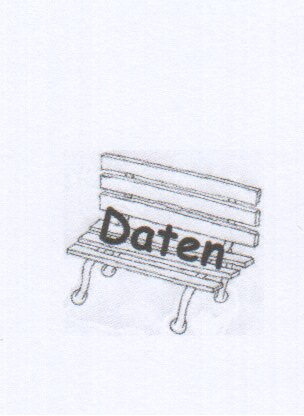
\includegraphics{Datenbank.jpg}
\caption{Datenbank}
\end{figure}

Mit Blick auf den potentiellen Adressatenkreis des Bandes bleibt auch
fraglich, ob es eine Lesergruppe gibt, der man einerseits einen Nachlass
als \enquote{Sammlung von Dokumenten oder anderen Dingen, die der
Verstorbene hinterlassen hat} (S. 96) erklären muss, der man
andererseits aber die Feinheiten der kooperativen überregionalen
Erschließung mittelalterlicher Originalhandschriften mit dem Ziel
erläutert, diese Handschriften lokalisieren und damit wissenschaftlich
arbeiten zu können (S. 93-96).

Stellt man fest, dass als einzige Online-Quellenedition zum 20.
Jahrhundert die bei De Gruyter erschienene Datenbank
\enquote{Nationalsozialismus, Holocaust, Widerstand und Exil 1933-1945}
präsentiert wird (S. 73), und liest man Sätze wie \enquote{Für die
Geistes- und Sozialwissenschaften bietet z. B. der Verlag De Gruyter
geschichtswissenschaftliche Zeitschriften im Volltext auf seiner
Online-Plattform an.} (S. 35), sieht man vor seinem geistigen Auge die
Marketing-Abteilung bei der Arbeit. Nachhaltigere Verkaufsförderung wäre
es möglicherweise gewesen, das Ressourcenverzeichnis (S. 127-131) besser
mit dem Text abzugleichen, fehlen darin doch u.a. die digitale Version
der International Bibliography of Historical Sciences (S. 21) oder die
als Beispiel für eine Personalbibliographie angeführte Helmut Schmidt
Bibliographie (S. 53).

Bevor sich der Rezensent nun endgültig in die Schwächen des Bandes
verbeißt, gilt es, den ersten der \enquote{Tipps für den absoluten
Notfall} zu beherzigen: \enquote{Nerven behalten und ruhig bleiben!} (S.
18). Die meisten, wenn nicht alle, der kritisierten Punkte dürften
weniger der Autorin anzulasten sein als vielmehr dem Konzept der Reihe.
Die aufgeworfenen Themen und die vorgestellten Ressourcen sind relevant
und sinnvoll ausgewählt. Bei einer Neuauflage sollten jedoch inhaltliche
Präzision und Lesbarkeit des Textes neu austariert werden. Auch
Studierenden ist zuzutrauen, dass sie komplexere Sachverhalte verstehen.

\begin{center}\rule{3in}{0.4pt}\end{center}

\textbf{Stefan Wiederkehr}, Dr.~phil., studierte Geschichte, Russische
Sprach- und Literaturwissenschaft sowie Philosophie in Zürich und
absolvierte den postgradualen Fernstudiengang Bibliotheks- und
Informationswissenschaft an der Humboldt-Universität zu Berlin. Seit
2009 ist er Leiter der Akademiebibliothek und Arbeitsstellenleiter des
Akademienvorhabens \enquote{Jahresberichte für deutsche Geschichte} an
der Berlin-Brandenburgischen Akademie der Wissenschaften.

\end{document}